

\documentclass[a4paper, 11pt, english, fleqn]{article}
\usepackage[utf8]{inputenc}
\usepackage{babel}
%\usepackage{ngerman}
\usepackage{coordsys,logsys,color}
\usepackage{fancyhdr}
\usepackage{hyperref}
\usepackage{texdraw}				
\usepackage[T1]{fontenc}					
\usepackage{amsmath,amsfonts,amssymb}	
\usepackage[normalem]{ulem}	
\usepackage{listings}
\usepackage{graphicx}
\usepackage{enumitem}
\usepackage[paper=a4paper,left=35mm,right=35mm,top=35mm,bottom=30mm]{geometry}

\hypersetup{colorlinks=true, breaklinks=true, linkcolor=darkblue, menucolor=black, urlcolor=darkblue, citecolor=darkblue}

\pagestyle{fancy}

\renewcommand{\familydefault}{cmss}

\definecolor{fgcgray}{rgb}{0.4, 0.4, 0.4}
\definecolor{darkblue}{rgb}{0,0, 0.4}
\newcommand{\titlefont}[1]{\textcolor{black}{\fontseries{bx}\fontshape{n}\fontsize{30}{0pt} \selectfont #1}}
\newcommand{\titlepagef}[1]{\textcolor{black}{\fontseries{bx}\fontshape{n}\fontsize{14}{0pt} \selectfont #1}}

\newcommand{\gloss}[1]{\textcolor{glossb}{\fontsize{11}{0pt}\selectfont #1}}

\newlist{aims}{enumerate}{1}
\setlist[aims,1]{
	label={Aim~\arabic*},
	leftmargin=*,
	align=left,
	%labelsep=1mm,
	font=\bfseries
}

\addtolength{\oddsidemargin}{-1.0cm}
\addtolength{\evensidemargin}{-1.0cm}
\addtolength{\headwidth}{2.0cm}
\addtolength{\textwidth}{2.0cm}

\setlength{\parindent}{0cm}

\renewcommand{\labelitemi}{$\circ$}
\renewcommand{\labelitemii}{$\diamond$}

\newcommand{\spaceline}[1][8pt]{\vskip #1}
\newcommand{\attrname}[1]{\textcolor{fgcgray}{\scriptsize #1}}

\newcommand{\comment}[1]{\spaceline[5pt] \textcolor{fgcgray}{\scriptsize #1} \spaceline[15pt]}

\makeatletter

\newcommand*{\project}[1]{\gdef\@project{#1}}


\def\@maketitle{
  %\begin{titlepage}
   
  \begin{center}
      \titlepagef{Software-Project 2017}
      \spaceline
  \end{center}
  
  \begin{center}
      \parbox{\textwidth}{
        \spaceline
        \centering{\titlefont{Detailed Design}}
        \par
        \spaceline
      }
  \end{center}
  
  \begin{center}
  	\titlepagef{Real-Time Mesh Utilities}
  	\spaceline[2em]
  \end{center}
  
  \begin{center}
  \begin{tabbing}
  Petros Simidyan \qquad \=
  Blerta Hamzallari \qquad \=
  Felix Griesau \qquad \=
  Marco Klamke \\
  Julius Lerm
  \>Lars Debor
  \>Simon Heinke  
  \>Sugandha Sachdeva
  \end{tabbing}
  \end{center}
 
  
  \spaceline[3em] {
    \begin{flushright}
    \begin{tabular}[t]{rl}
      \attrname{last change:} & \@date
    \end{tabular}
    \end{flushright}
    \par
  }
  \spaceline[5.5em]
  %\end{titlepage}
}

\begin{document}

\pagenumbering{gobble}
	
\lhead{\sc{Detailed Design: RTMU}}	
\title{Detailed Design: RTMU}
\vspace{3 in}
\maketitle


\includegraphics[width = \linewidth]{figures/mne-cpp.png}

\clearpage

\pagenumbering{arabic}

\tableofcontents

\clearpage
\section{General Architecture}
The features of the Real-Time Mesh Utilities are distributed onto two classes: the Surface Constrained Distance Calculation (from now on abbreviated with SCDC) and the Sensor Projecting can be found inside class \textbf{GeometryInfo}, while the Interpolation is housed inside class \textbf{Interpolation}.\\
Both classes lie within the library layer of MNE-CPP:

\begin{figure}[h]
	\begin{center}
		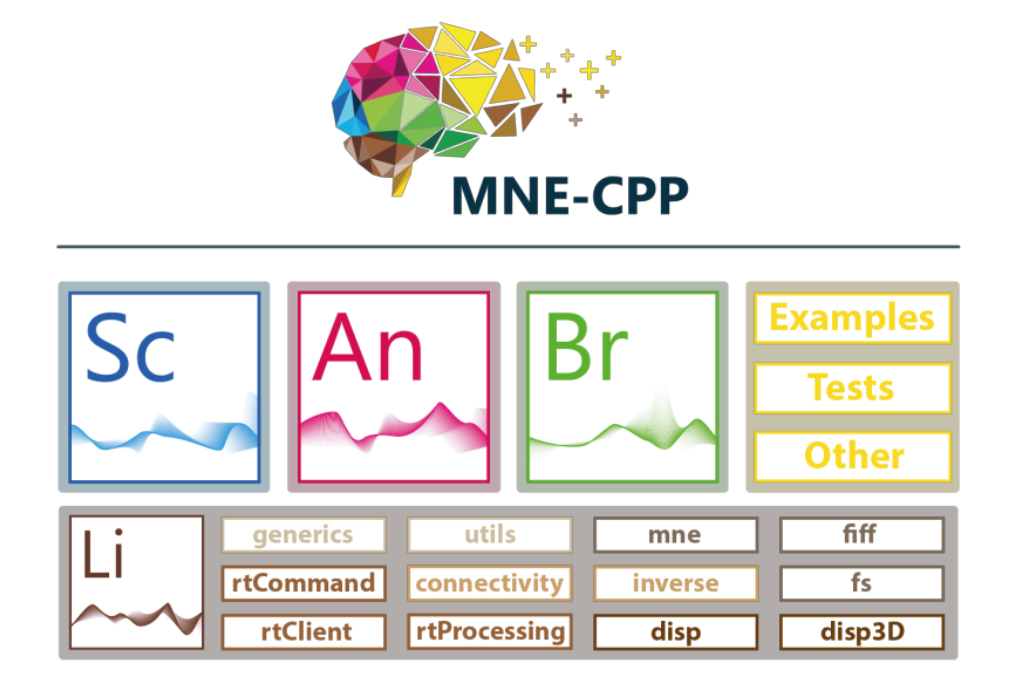
\includegraphics[width=10cm]{figures/mne_architecture.png}
		\caption{Overview of the MNE-CPP basic architectural layout}
	\end{center}
\end{figure}

The classes are to be used by the application layer which includes all front end applications (i.e. MNE Scan, MNE Analyze and MNE Browse).
The added functionality thus extends the preexisting framework.\\
For a seamless integration into mentioned front-end applications, the new features will be added to the hierarchical GUI structure of MNE-CPP. This requires for a so called DataTreeItem to be created. The latter will allow easy modification of parameters of the two classes (see detailed class descriptions for more details). By the time this document was written the DataTreeItem was not functional yet, thus it is not included in this document.


\clearpage

\section{GeometryInfo}

The class \textbf{GeometryInfo} holds all needed functionality for the SCDC and the Sensor Projecting (see Functional Specification for further details). Since all included methods are static, the class itself does not have to be instantiated, thus it also is declared static and the default constructor is forbidden.\\
The class \textbf{GeometryInfo} does not have any class members.

\begin{figure}[h]
	\begin{center}
		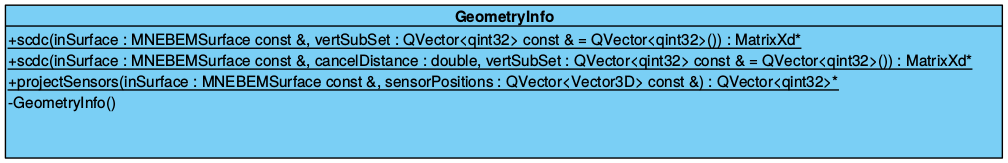
\includegraphics[width=16cm]{figures/geometryinfoclassdiagram.png}
		\caption{Interface of GeometryInfo}
	\end{center}
\end{figure}

\subsection{Member Functions}

\subsubsection{scdc}
The method \textbf{scdc} originally was thought to receive only one input argument, i.e. the MNEBemSurface (object that holds the needed adjacency information). Based on this, it was supposed to calculate the full distance table of all contained vertices. Since the latter would have needed around 160 gigabytes of memory for some meshes, it was decided that the method also receives a subset of vertices. It then only calculates all distances for each vertex of said subset. The subset argument is defaulted with an empty vector, in case a subset could not be provided or is not wanted.\\
After first tests revealed that an unrestricted distance calculation would take far too long, a third argument was introduced: a double-value that acts as a distance threshold and thus restricts the distance calculation to vertices which lie within the said radius. This seems a bit imprecise or careless at first glance, but it actually is reasonable for this specific application: bilateral stimulation of cells inside the brain only occurs up to a certain distance. The third argument is defaulted with the maximum double-value, in case a distance threshold could not be provided or is not wanted.\\
After these restrictions and adaptions were agreed upon, the question which algorithm to choose arose.
While Pettie and Ramachandrans algorithm had the best asymptotic run-time, further research revealed that an implementation would go far beyond the scope of this project, since the algorithm uses several other subroutines (such as Prims method for minimal spanning trees). Another possible candidate for solving the problem was Thorups algorithm. Testing of a publicly available implementation showed that it actually did worse than another algorithm, when the above mentioned restrictions to the problem were applied. The only algorithm that resulted in a lower computation time was an iterative version of Dijkstra's algorithm (see below for more details).\\
The \textbf{scdc} method allocates the necessary memory and initializes the distance table.
Since two instances of \textbf{iterativeDijkstra} would not interfere with each other (because they work on different columns of the distance table), it was decided for \textbf{scdc} to start several threads. According to the number of available threads (or cores, depending on hyperthreading etc.), the passed subset of vertices gets split into equally sized parts, whose limiting indices are then passed to an instance of \textbf{iterativeDijkstra}. The \textbf{scdc} method then was supposed to wait for all threads to finish by using a periodic check, so it could return the filled distance table to the caller.\\
To further improve performance, this procedure was slightly changed: one instance of \textbf{iterativeDijkstra} gets executed on the main thread, i.e. the thread that called \textbf{scdc}. This avoids unnecessary thread changes for the periodic check and in that way decreases computation time.

\clearpage

\begin{figure}[h]
	\begin{center}
		\includegraphics[width=16cm]{figures/scdc_seq.png}
		\caption{Sequence diagram of method \textbf{scdc}. Arguments to calls are not included to ensure readability}
	\end{center}
\end{figure}

\subsubsection{iterativeDijkstra}
The method \textbf{iterativeDijkstra} receives six input arguments: Firstly a pointer to the distance table which the results are to be written into. Secondly a reference to a MNEBemSurface holds the necessary adjacency information. As described above, the \textbf{iterativeDijkstra} method receives a vector of indices which point to vertices inside the MNEBemSurface. Added to that, it gets passed two indices which limit the section of said vector that the respective instance of \textbf{iterativeDijkstra} is responsible for.\\
Since the external requirements (i.e. low computation time and overall high efficiency) induce some restrictions (see description of \textbf{scdc} for more details), a distance threshold gets passed as the sixth argument. Because Dijkstra's algorithm is so well known, its general implementation is not described in this document. Apart from a standard version of Dijkstra's algorithm, \textbf{iterativeDijkstra} ignores vertices that have a higher distance than said threshold, that means it does not check their neighbors for possibly better paths.\\
This method is private since it only gets called by \textbf{scdc} as a subroutine and is not part of the external interface of class \textbf{GeometryInfo}.

\subsubsection{projectSensors}
The method \text{projectSensors} receives two input arguments: A MNEBemSurface for the adjacency information and a vector of sensor positions in 3D space. It was intended for \textbf{projectSensors} to use a k-D tree for fast lookups during the mapping of sensors. After the k-D tree was implemented, it was striking that average times for a lookup (which should be logarithmic in theory) were far too slow to sustain an overall efficient run-time of the program. Added to that, the method for building the tree could only be executed on one thread, since the structural dependencies within a k-D tree are far to complicated to be divided onto two ore more threads.\\
A simple linear search that finds the minimal distance between any vertex of the mesh and the respective sensor resulted in a better run-time. Although this was originally thought of as a verification tool due to its simplicity, it was then extended and optimized.\\
Since two instances of linear search would not interfere with each other, it was decided for \textbf{projectSensors} to start several threads.
According to the number of available threads (or cores, depending on hyperthreading etc.), the passed vector of sensor positions gets split into equally sized parts, whose limiting iterators are then passed to an instance of \textbf{nearestNeighbor}. Each instance returns a vector of IDs which refer to vertices of the mesh. The \textbf{projectSensors} method was supposed to wait for all threads to finish by using a periodic check, so it could append the resulting vectors in the right order and return the outcome to the caller.\\
To further improve performance, this procedure was slightly changed: one instance of \textbf{nearestNeighbor} gets executed on the main thread, i.e. the thread that called \textbf{projectSensors}. This avoids unnecessary thread changes for the periodic check and thus decreases computation time.

\clearpage

\begin{figure}[h]
	\begin{center}
		\includegraphics[width=16cm]{figures/projectsensors_seq.png}
		\caption{Sequence diagram of method \textbf{projectSensors}. Arguments to calls are not included to ensure readability}
	\end{center}
\end{figure}

\clearpage

\subsubsection{nearestNeighbor}
The method \textbf{nearestNeighbor} receives three input arguments: A MNEBemSurface, and two iterators. The first iterator points to the start and the second to the end of a section of a vector.
It then iterates over every sensor position between the two iterators and searches for the vertex with the closest distance to the respective sensor. In order to achieve this, it compares the distances of all vertices stored inside the MNEBemSurface. After a shortest distance is found for a specific sensor, the ID of the corresponding vertex is pushed back into a result vector. After the limiting iterator has been reached, this result vector is then returned to the caller.\\
This method is private, since it only gets called by \textbf{projectSensors} as a subroutine and is not part of the external interface of class \textbf{GeometryInfo}.

\subsubsection{matrixDump}
This method is implemented for testing and verifying purposes only. It receives a matrix and a string. It then writes the content of the matrix into a file that is named with said string.

\subsubsection{squared}
This method is implemented for better readability only, thus it is declared private. It receives a double-value and returns it squared. In order to avoid efficiency losses through stack frames, it is declared inline.

\clearpage


\section{Interpolation}
The class \textbf{Interpolation} holds all needed functionality to create a weight matrix based on a distance table and to interpolate sensor signals. Since all included methods are static, the class itself does not have to be instantiated, therefore it also is declared static and the default constructor is forbidden.

\begin{figure}[h]
	\begin{center}
		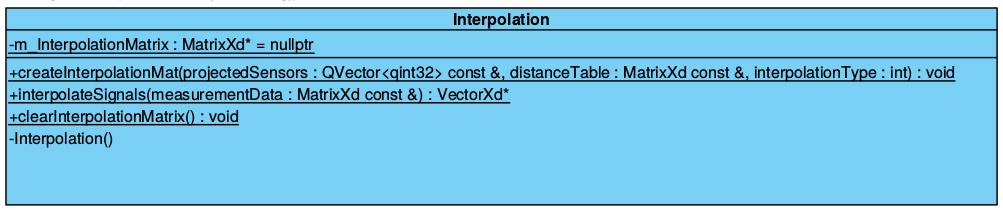
\includegraphics[width=16cm]{figures/interpolationclassdiagram.png}
		\caption{Interface of Interpolation}
	\end{center}
\end{figure}

\subsection{Member Objects}

\subsubsection{Weight Matrix}
The class \textbf{Interpolation} holds one static class member: \textbf{m\_interpolationMatrix} which is a shared pointer to a sparse matrix (i.e. the weight matrix). Since a user of the \textbf{Interpolation} class does not care about internal representation of the weight matrix and is only interested in fast interpolation of signals, it was decided that the weight matrix should be stored as a member of the class. In case access to the matrix itself should be needed, a designated \textbf{getter}-function was included (see method \textbf{getResult} for more details).\\
Originally, this member was supposed to be of type \textbf{Eigen::MatrixXd} which is a standard matrix of double-values with variable dimensions. After first tests revealed that depending on the distance threshold chosen during the calculation of distances on the mesh (see section 2.1.1) the weight matrix contained around 97\% of null-entries, the weight matrix was changed to type \textbf{Eigen::SparseMatrix<double>} which is optimized for sparse matrices. This implied some changes to the calculation of the weight matrix within the method \textbf{createInterpolationMat} because \textbf{Eigen::\ SparseMatrix<double>} do not provide the same interface as \textbf{Eigen::MatrixXd}.

\subsection{Member Functions}

\subsubsection{createInterpolationMat}
The method \textbf{createInterpolationMatrix} receives four input arguments: Firstly a vector of IDs which represent the vertices which have been assigned to a sensor during the Sensor Projecting (see section 2.1.3 for more details). Secondly a shared pointer to a distance table, i.e. a matrix of double-values.\\
Since the weight matrix can be calculated using a variety of mathematical interpolation functions (e.g. a linear function, a quadratic function, etc.), the method \textbf{createInterpolationMat} was thought to receive some kind of value to represent the chosen function. That could for example be achieved by defining global constants and encoding the functions with them. For a higher level of versatility it was decided that \textbf{createInterpolationMat} should receive a pointer to a function, which in turn receives a double-value and returns a double-value and thus fulfills the internal requirements of the weight matrix calculation. A minimal preset of usable functions was provided as public members of the class (see section 3.2.5 for more details).\\
Since bilateral stimulation of cells in the brain only occurs up to certain distances, a double-value is received as a fourth argument. It acts as a distance threshold, that means that the interpolation weight of vertices with a higher distance than said threshold is set to zero. 

\subsubsection{interpolateSignal}
The method \textbf{interpolateSignal} receives a vector of double values which represents a specific moment of brain activity, i.e. the values that were recorded by sensors. The weight matrix gets multiplied with the input vector and thus produces a vector that contains the brain activity for all vertices of the distance table that was used to create the weight matrix.

\subsubsection{clearInterpolationMatrix}
The method \textbf{clearInterpolationMatrix} resets the weight matrix, i.e. frees all memory allocated for the respective member object.
\\\\

\begin{figure}[h]
	\begin{center}
		\includegraphics[width=16cm]{figures/interpolation_seq.png}
		\caption{Sequence diagram for class \textbf{Interpolation}. Arguments to calls are not included to ensure readability}
	\end{center}
\end{figure}

\subsubsection{getResult}
This method is implemented in case the calculated weight matrix is needed as an object itself. It returns a smart pointer to the weight matrix.

\subsubsection{linear, gaussian, square}
These methods are implemented to provide a minimal preset of functions to use during the calculation of the interpolation weight matrix (see method \textbf{createInterpolationMatrix} for more details).

\clearpage

\section{Glossary}

\begin{aims}
	
	\item[Mesh] describes the representation of a planar graph in 3D space.
	\item[Eigen] is a C++ template library for linear algebra that includes matrices, vectors, numerical solvers, and related algorithms
	\item[MatrixXd] is a specialized class from the Eigen framework. It represents a matrix of double-values (MatrixX\textbf{d}) that has variable dimensions (Matrix\textbf{X}d)
	\item[SparseMatrix<T>] is an optimized version of standard Eigen matrices that is designated for sparse matrices.
	\item[MNEBemSurface] is a class from the MNE-CPP framework that holds information about the represented surface and its geometry.
	\item [SCDC] (surface constrained distance calculation) determines the shortest path between two points on a tessellated surface.
	\item [MNE-CPP] is a cross-platform C++ framework, which provides MEG/EEG tools and applications for fast non-invasive brain monitoring.
	\item[Pettie and Ramachandran] Seth Pettie and Vijaya Ramachandran published their paper "A Shortest Path Algorithm for Real-Weighted Undirected Graphs" in 2005.
	\item[Prim] Robert C. Prim had republished a previously known algorithm for finding minimal spanning trees in 1957.
	\item[Thorup] Mikkel Thorup is a computer scientist who published his algorithm for solving the single source shortest path problem in 1997.
	\item[Dijkstra] Edsger W. Dijkstra was a computer scientist who published his algorithm for solving the single source shortest path problem in 1959.
	\item [Linear search] or sequential search is a method for finding a target value within a list.
\end{aims}

  
\end{document}
